\section{Resultados}
% Deben incluir los resultados de los experimentos, utilizando el formato mas
% adecuado para su presentacion. Deberan especicar claramente a que
% experiencia corresponde cada resultado. No se incluiran aqu corridas de
% maquina. Algo fundamental en su aprendizaje en la materia es la presentacion
% de resultados de forma clara y concisa para el lector

\subsection{Experimento 1: Aumentar el span}

Para este tipo de experimento lo que hicimos fue fijar todos los parámetros e incrementar el $span$. El propósito de esta prueba era observar como iba evolucionando la fuerza máxima aplicada en los links.\\

Nuestro set de datos será: $n = 8$, $h = 3$ y $C_i = 5$ para $i \in [1 \dots 7]$\\

Nuestra hipótesis basada simplemente en el instinto es que las fuerzas irían aumentando a medida que el $span$ aumenta, ya que la longitud por cada sección aumenta haciendo que los links tengan que soportar mas peso. Veamos lo que realmente sucede:

\begin{center}
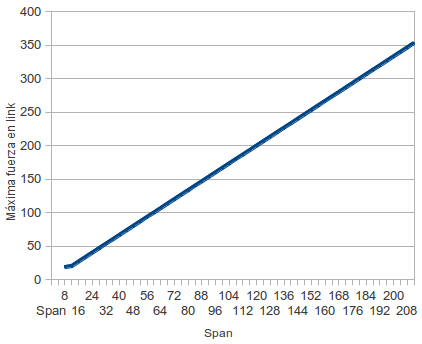
\includegraphics[scale=0.8]{archivos/graficos/Fuerza-x-span.png}\\
Evolución de la fuerza máxima a medida que crece el $span$
\end{center}

Podemos ver que la fuerza mayor está en $f_{14}$ hasta que el ancho de la sección es de 5,5 (donde el ratio de ancho vs. altura es de 1,83), luego pasa a ser $f_2$.\\

$f_{14}$ es la viga superior izquierda central (como el puente es simétrico y cualquier asimetría se debe a pequeños errores numéricos, el link $f_{18}$ tiene un valor idéntico).\\

Esto indica que, para puentes con secciones más altas que anchas, la vigas superiores centrales se comprimen al soportar todo el peso del puente en una forma desproporcionada.\\

Conforme la sección se hace más ancha, esa carga parece disminuir, hasta que la vigas que soportan más peso son las diagonales extremas, que cargan todo el peso del puente consigo.\\

Y como se puede observar la fuerza máxima disminuye, contrariamente a lo que habíamos formulado en un principio. A la luz de los resultados creemos que esto puede deberse a que a medida que el $span$ crece los angulos en los links diagonales se van achicando haciendo que al multiplicar por las fuerzas, el valor numérico de estas disminuya.

\subsection{Experimento 2: Aumentar el span, pero fijando una carga central}

\begin{center}
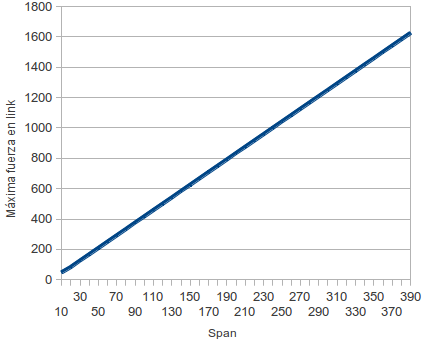
\includegraphics[scale=0.8]{archivos/graficos/Fuerza-x-span2.png}\\
Evolución de la fuerza máxima a medida que crece el $span$ con un peso central
\end{center}
